\let\negmedspace\undefined
\let\negthickspace\undefined
\documentclass[journal]{IEEEtran}
\usepackage[a5paper, margin=10mm, onecolumn]{geometry}
%\usepackage{lmodern} % Ensure lmodern is loaded for pdflatex
\usepackage{tfrupee} % Include tfrupee package

\setlength{\headheight}{1cm} % Set the height of the header box
\setlength{\headsep}{0mm}     % Set the distance between the header box and the top of the text

\usepackage{gvv-book}
\usepackage{gvv}
\usepackage{cite}
\usepackage{amsmath,amssymb,amsfonts,amsthm}
\usepackage{algorithmic}
\usepackage{graphicx}
\usepackage{textcomp}
\usepackage{xcolor}
\usepackage{txfonts}
\usepackage{listings}
\usepackage{enumitem}
\usepackage{mathtools}
\usepackage{gensymb}
\usepackage{comment}
\usepackage[breaklinks=true]{hyperref}
\usepackage{tkz-euclide} 
\usepackage{listings}
% \usepackage{gvv}                                        
\def\inputGnumericTable{}                                 
\usepackage[latin1]{inputenc}                                
\usepackage{color}                                            
\usepackage{array}                                            
\usepackage{longtable}                                       
\usepackage{calc}                                             
\usepackage{multirow}                                         
\usepackage{hhline}                                           
\usepackage{ifthen}                                           
\usepackage{lscape}
\begin{document}

\bibliographystyle{IEEEtran}
\vspace{3cm}

\title{9-9.2-26}
\author{AI24BTECH11015 - Harshvardhan Patidar}
 \maketitle
% \newpage
% \bigskip
{\let\newpage\relax\maketitle}

\renewcommand{\thefigure}{\theenumi}
\renewcommand{\thetable}{\theenumi}
\setlength{\intextsep}{10pt} % Space between text and floats


\numberwithin{equation}{enumi}
\numberwithin{figure}{enumi}
\renewcommand{\thetable}{\theenumi}

Question: \\
	Find the area of the region included between $y^2 = 9x$ and $y = x$.

\solution \\
	\begin{table}[h!]    
  		\centering
  		\begin{tabular}[12pt]{ |c| c|}
    \hline
    \textbf{Variable} & \textbf{Description}\\
    \hline
	$\vec{m}$ & Unit Vector\\
    \hline
	$\alpha$ & Angle of the unit vector with $x$-axis\\
    \hline
	$\beta$ & Angle of the unit vector with $y$-axis\\
    \hline	
    \end{tabular}

  		\caption{Variables Used}
  		\label{tab1-1.9-6}
	\end{table}\\

	The general equation of a parabola with directrix $\vec{n}^{\top}\vec{x}=c$ is given by,
	\begin{align}
		g\brak{\vec{x}}=\vec{x}^{\top}\vec{V}\vec{x}+2\vec{u}^{\top}\vec{x}+f=0\\
		\vec{V}=\norm{\vec{n}}^2\vec{I}-e^2\vec{n}\vec{n}^{\top}\\
		\vec{u}=ce^2\vec{n}-\norm{\vec{n}}^2\vec{F}\\
		f=\norm{\vec{n}}^2\norm{\vec{F}}^2-c^2e^2
	\end{align}

	For the parabola $y^2=4x$, equation of directrix is, $\myvec{-1&0}\vec{x}=\frac{9}{4}$
	\begin{align}
		\vec{V}&=\myvec{0&0\\0&1}\\
		\vec{u}&=\myvec{-\frac{9}{2}\\0}\\
		f&=0
	\end{align}

	The line parameters are 
	\begin{align}
		\vec{h} &= \myvec{0\\0} , \vec{m} = \myvec{1\\1}
	\end{align}

	The point of intersection of a Line and a conic are given by 
	\begin{align}
		\vec{x} = \vec{h} + \kappa_i \vec{m}
	\end{align}
	
	where
	\begin{align}
		\kappa_{i} = \frac{1}{\vec{m}^{\top} \vec{V} \vec{m}} \brak{-\vec{m}^\top \brak{\vec{V} \vec{h} + \vec{u}} \pm \sqrt{\sbrak{\vec{m}^\top \brak{\vec{V} \vec{h} + \vec{u}}}^2 - g\brak{\vec{h}} \brak{\vec{m}^\top \vec{V} \vec{m}}}}
	\end{align}

	On solving we get the points of intersection to be \myvec{0\\0} , \myvec{9\\9}. Area between the line and the parabola is,
	\begin{align}
		\int_0^9 3\sqrt{x}dx - \int_0^9 x dx = \frac{27}{2}
	\end{align}

	So, the area between the parabola $y^2 = 9x$ and line $y=x$ is $\frac{27}{2}$

	\begin{figure}[h!]
   		\centering
   		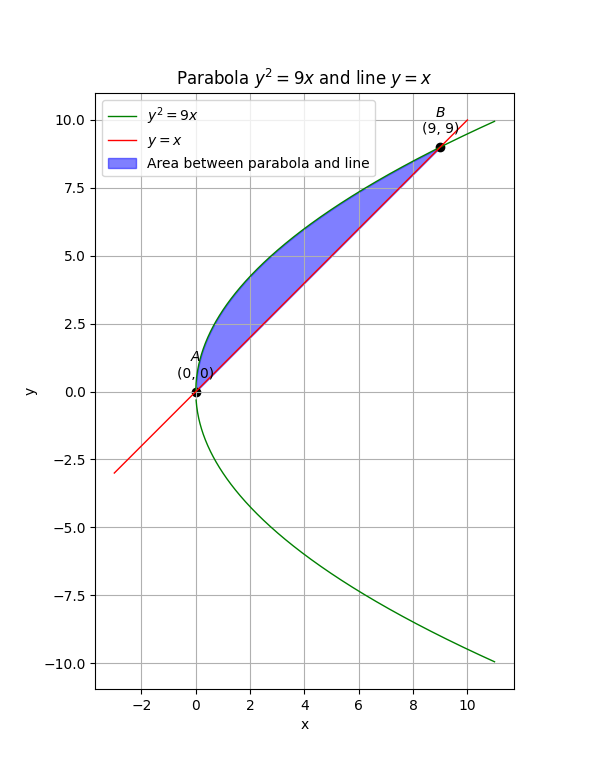
\includegraphics[width = 1\linewidth]{plots/plot.png}
   		\caption{}
   		\label{stemplot}
	\end{figure}
\end{document}


